% !TEX root = main.tex
%
% Label Theory
%
We shall now define the functions labeling the transitions of SW automata and transducers,
generalizing the Boolean algebras of~\cite{dAntoniVeanes17CAV}
from Boolean to other semiring domains.
%
We consider \emph{alphabets}, which are countable sets of symbols
denoted $\Sigma$, $\Delta$,...
\florent{ADD: notations $\Sigma^*$, $\varepsilon$...}
%Let $\< \Semiring, \oplus, \zero, \otimes, \one>$ be a commutative, complete semiring.
%
\noindent
Given a semiring $\< \Semiring, \oplus, \zero, \otimes, \one>$,
a \emph{label theory} over $\Semiring$
is a set $\bar\Phi$ of recursively enumerable sets denoted
%$\Phi_\epsilon \subseteq \Semiring$, % containing constant functions valued in $\Semiring$,
$\Phi_\Sigma$, %and $\Phi_\Delta$,
containing unary functions of type $\Sigma \to \Semiring$, %resp. $\Delta \to \Semiring$,
or $\Phi_{\Sigma, \Delta}$, containing binary functions $\Sigma \times \Delta \to \Semiring$,
and such that:
\florent{unary for \SWA (weight depends on input symbol) 
         and binary for transducers and VPA (weight depends on input symbol AND output or stack symbol)} 

\noindent --
for all $\Phi_{\Sigma, \Delta} \in \bar\Phi$, we have
$\Phi_{\Sigma} \in \bar\Phi$ and $\Phi_{\Delta} \in \bar\Phi$

\noindent --
every $\Phi_{\Sigma}\in \bar\Phi$ contains all the constant functions from $\Sigma$ into $\Semiring$,

\noindent --
for all $\alpha \in \Semiring$ and $\phi \in \Phi_\Sigma$,
      $\alpha \otimes \phi : x \mapsto \alpha \otimes \phi(x)$,
      and $\phi \otimes \alpha : x \mapsto \phi(x) \otimes \alpha$\\
\phantom{--} belong to $\Phi_\Sigma$, and similarly for $\oplus$
      and for $\Phi_{\Sigma, \Delta}$

\noindent --
for all $\phi, \phi' \in \Phi_\Sigma$,
$\phi \otimes \phi': x \mapsto \phi(x) \otimes \phi'(x)$ belongs to $\Phi_\Sigma$

\noindent --
for all $\eta, \eta' \in \Phi_{\Sigma, \Delta}$
$\eta \otimes \eta': x, y \mapsto \eta(x, y) \otimes \eta'(x, y)$ belongs to $\Phi_{\Sigma, \Delta}$

\noindent --
for all $\phi \in \Phi_\Sigma$ and $\eta \in \Phi_{\Sigma, \Delta}$,
$\phi \otimes_1 \eta: x, y \mapsto \phi(x) \otimes \eta(x, y)$ and\\
\phantom{--} $\eta \otimes_1 \phi: x, y \mapsto \eta(x, y) \otimes \phi(x)$
belong to $\Phi_{\Sigma, \Delta}$

\noindent --
for all $\psi \in \Phi_\Delta$ and $\eta \in \Phi_{\Sigma, \Delta}$,
$\psi \otimes_2 \eta: x, y \mapsto \psi(y) \otimes \eta(x, y)$ and\\
\phantom{--} $\eta \otimes_2 \psi: x, y \mapsto \eta(x, y) \otimes \psi(y)$
belong to $\Phi_{\Sigma, \Delta}$

\noindent --
similar closures hold for $\oplus$.

%\noindent --
%the partial applications $\eta \in \Phi_{\Sigma, \Delta}$
%and $\eta_a: y \mapsto \eta(a, y)$ for $a \in \Sigma$ %and $y \in \Delta$
%and\\
%\phantom{--} $\eta_b: x \mapsto \eta(x, b)$ for $b \in \Delta$ %and $x \in \Sigma$,
%belong respectively to~$\Phi_\Delta$ and~$\Phi_\Sigma$.
\florent{partial application is needed?}

%Moreover, these sets are required to be closed under the
%operators~$\oplus$ and~$\otimes$ of~$\Semiring$:
%for all $\phi, \phi' \in \Phi_\Sigma$,
%$\psi, \psi' \in \Phi_\Delta$,
%and $\eta, \eta' \in \Phi_{\Sigma, \Delta}$, %the function
%%
%\begin{center}
%\begin{tabular}{cclll}
%$\phi \otimes \phi'$ & : & $x \mapsto \phi(x) \otimes \phi'(x)$ & belongs to $\Phi_\Sigma$,\\
%$\psi \otimes \psi'$ & : & $y \mapsto \psi(y) \otimes \psi'(y)$ & belongs to $\Phi_\Delta$,\\
%$\phi \otimes \eta$\;  & : & $x, y \mapsto \phi(x) \otimes \eta(x, y)$ & belongs to $\Phi_{\Sigma, \Delta}$,\\
%$\eta \otimes \psi$  & : & $x, y \mapsto \eta(x, y) \otimes \psi(y)$ & belongs to $\Phi_{\Sigma, \Delta}$,\\
%$\eta \otimes \eta'$ & : & $x, y \mapsto \eta(x, y) \otimes \eta'(x, y)$ & belongs to $\Phi_{\Sigma, \Delta}$, &
%\multicolumn{1}{r}{and similarly for $\oplus$.}\\ %the same also holds for the binary sum operator $\oplus$.
%\end{tabular}
%\end{center}
%
%Finally, it is also required
%% that the codomain of every function of $\Phi_\Sigma$ and $\Phi_\Delta$
%% is a subset of $\Phi_\epsilon$, and
%that the partial applications of a function $\eta \in \Phi_{\Sigma, \Delta}$,
%resp.  $\eta_a: y \mapsto f(a, y)$ for $a \in \Sigma$ and $y \in \Delta$
%and  $\eta_b: x \mapsto f(x, b)$ for $b \in \Delta$ and $x \in \Sigma$,
%belong resp. to~$\Phi_\Sigma$ and~$\Phi_\Delta$.
%
\noindent
Intuitively, the operators $\bigoplus_\Sigma$
return global minimum, \wrt $\leq_\oplus$, of functions of~$\Phi_\Sigma$.
%
When the semiring $\Semiring$ is complete, we
consider the following operators on the functions of~$\bar\Phi$. % a label theory.
%(we use overloading to simplify notations):
\[
\begin{array}{ll}
\bigoplus_\Sigma : \Phi_\Sigma \to \Semiring,\
  \phi \mapsto \displaystyle\bigoplus_{a \in \Sigma} \phi(a)\\
\bigoplus^1_\Sigma :
  \Phi_{\Sigma,\Delta} \to \Phi_\Delta,\
  \eta \mapsto \bigl( y \mapsto \displaystyle\bigoplus_{a \in \Sigma} \eta(a, y) \bigr) &
\bigoplus^2_\Delta :
  \Phi_{\Sigma,\Delta} \to \Phi_\Sigma,\
  \eta \mapsto \bigl( x \mapsto \displaystyle\bigoplus_{b \in \Delta} \eta(x, b) \bigr)\\
\end{array}
\]
%
\medskip\noindent
In what follows, we might omit the sub- and superscripts in
$\otimes_1$, $\bigoplus^1_\Sigma$...,
%$\otimes_2$, $\oplus_1$, $\oplus_2$
when there is no ambiguity.
We shall keep them only for the special case $\Sigma = \Delta$,
\ie $\eta \in \Phi_{\Sigma, \Sigma}$, % for~$\otimes_1$ above,
%and $\eta \in \Phi_{\Delta, \Delta}$ for~$\otimes_2$.
%Similarly as for the above product and sum of functions,
%the superscripts in $\bigoplus^1_\Sigma$ and $\bigoplus^2_\Sigma$
%shall be reserved to the ambiguous case of $\Phi_{\Sigma,\Sigma}$,
in order to be able to distinguish between the first and the second argument.
%
\begin{definition}\label{def:label-th-complete}
A label theory~$\bar\Phi$ is \emph{complete} when
the underlying semiring~$\Semiring$ is complete, and
for all $\Phi_{\Sigma, \Delta} \in \bar\Phi$
and all $\eta \in \Phi_{\Sigma, \Delta}$,
$\bigoplus^1_\Sigma \eta \in \Phi_{\Delta}$ and
$\bigoplus^2_\Delta \eta \in \Phi_{\Sigma}$.
\end{definition}
%
\florent{notion of diagram of functions akin BDD for transitions in practice}

\noindent
The following facts are immediate.
\florent{mv appendix?}
%
\begin{lemma}
For $\bar\Phi$ complete %label theory for all
$\alpha \in \Semiring$,
$\phi, \phi' \in \Phi_{\Sigma}$,
$\psi \in \Phi_{\Delta}$, and
$\eta \in \Phi_{\Sigma, \Delta}$:
%
\begin{enumerate}
\item[$i.$]
\( \bigoplus_{\Sigma}\bigoplus^2_{\Delta} \eta = \bigoplus_{\Delta}\bigoplus^1_{\Sigma} \eta \)
\item[$ii.$]
\( \alpha \otimes \bigoplus_{\Sigma} \phi = \bigoplus_{\Sigma} (\alpha \otimes \phi) \) and
\( \bigl( \bigoplus_{\Sigma} \phi \bigr) \otimes\alpha = \bigoplus_{\Sigma} (\phi \otimes \alpha) \),
and similarly for~$\oplus$
\item[$iii.$]
\( \bigl(\bigoplus_{\Sigma} \phi\bigr) \oplus \bigl(\bigoplus_{\Sigma} \phi'\bigr)
   = \bigoplus_{\Sigma} (\phi \oplus \phi') \) and
\( \bigl(\bigoplus_{\Sigma} \phi\bigr) \otimes \bigl(\bigoplus_{\Sigma} \phi'\bigr)
   = \bigoplus_{\Sigma} (\phi \otimes \phi') \)
\item[$iv.$]
\( \bigl(\bigoplus^2_{\Delta} \eta\bigr) \oplus \bigl(\bigoplus^2_{\Delta} \eta' \bigr) =
 \bigoplus^2_{\Delta} (\eta \oplus \eta') \), and
\( \bigl(\bigoplus^2_{\Delta} \eta\bigr) \otimes \bigl(\bigoplus^2_{\Delta} \eta' \bigr) =
 \bigoplus^2_{\Delta} (\eta \otimes \eta') \)
\item[$v.$]
%\( \phi \oplus \bigl(\bigoplus_{\Delta} \eta\bigr) = \bigoplus_{\Delta} (\phi \oplus \eta) \),
\( \phi \otimes \bigl(\bigoplus^2_{\Delta} \eta\bigr) = \bigoplus_{\Delta} (\phi \otimes_1 \eta) \), and
\( \bigl(\bigoplus^2_{\Delta} \eta\bigr) \otimes \phi = \bigoplus_{\Delta} (\eta \otimes_1 \phi) \),
and similarly for~$\oplus$
\item[$vi.$]
%\( \psi \oplus \bigl(\bigoplus_{\Sigma} \eta\bigr) = \bigoplus_{\Sigma} (\psi \oplus \eta) \),
\( \psi \otimes \bigl(\bigoplus^1_{\Sigma} \eta\bigr) = \bigoplus_{\Sigma} (\psi \otimes_2 \eta) \), and
\( \bigl(\bigoplus^1_{\Sigma} \eta\bigr) \otimes \psi = \bigoplus_{\Sigma} (\eta \otimes_2 \psi) \),
and similarly for~$\oplus$
\end{enumerate}
\end{lemma}

%we call \emph{summary} of a function
%$\phi \in \Phi_\Sigma$,
%resp. $\eta \in \Phi_{\Sigma, \Delta}$,
%the value $\bigoplus_{a \in \Sigma} \phi(a)$,
%resp. $\bigoplus_{a \in \Sigma} \bigoplus_{b \in \Delta} \eta(a, b)$.
%By definition of infinite sums in complete semirings,
%a summary of $\phi \oplus \phi'$, $\alpha \otimes \phi$ and $\phi \otimes \alpha$
%can be computed from $\alpha \in \Semiring$ and summaries of $\phi$ and $\phi'$ in $\Phi_{\Sigma}$,
%using the operators of $\Semiring$,
%and the same holds for $\Phi_{\Delta}$ and $\Phi_{\Sigma, \Delta}$.


\philippe{Je trouve qu'il y a beaucoup de notions à retenir (complete, effective) et ça devient
difficile pour un lecteur non spécialiste. Est-ce que tout est nécessaire (je ne sais plus qui m'avait dit:
un concept en plus, un point en moins.}

\noindent
A label theory is called \emph{effective} when
for all $\phi \in \Phi_\Sigma$ and $\eta \in \Phi_{\Sigma, \Delta}$,
$\bigoplus_{\Sigma} \phi$,
$\bigoplus_{\Delta}\bigoplus_{\Sigma} \eta$, and
$\bigoplus_{\Sigma}\bigoplus_{\Delta} \eta$
can be effectively computed from $\phi$ and $\eta$.
\florent{$\exists$ oracle returning ...  in worst time complexity $T$.}


%there is an oracle returning, in constant time,
%$\bigoplus_{\Sigma} \phi$,
%$\bigoplus_{\Sigma} \eta$, and
%$\bigoplus_{\Delta} \eta$
%and one symbol where the function reaches this minimum,
%denoted $\bigominus_\Sigma \phi$

%\begin{definition}\label{def:label-th-convex}
%Let $\Omega$ be an alphabet
%A function $\phi \in \Phi_\Sigma$ in a label theory over a complete semiring $\Semiring$
%is called $k$-\emph{convex}, for a natural number $k$, iff
%$\mathrm{card}\{ a \in \Sigma \mid \phi(a) = \bigoplus_{\Sigma} \phi \} \leq k$.
%\end{definition}
%A label theory is $k$-convex if all its functions are $k$-convex.

%s.t. for all $\phi \in \Phii$,
%$\psi \in \Phir$,
%and $\eta \in \Phicr$,
%$\displaystyle\bigoplus_{a \in \Omegai} \phi(a)$
%$\displaystyle\bigoplus_{r \in \Omegar} \phi(r)$ and
%$\displaystyle\bigoplus_{{\call{c}} \in \Omegac}
%\displaystyle\bigoplus_{{\return{r}} \in \Omegar} \eta({\call{c}}, {\return{r}})$
%are computable...
%
% total ?
% monotonic and superior writ natural ordering
%Regarding the infinite sum operator, note that
%$\bigoplus_{x \in \Phi_\Omega} \phi(x)$,
%$\bigoplus_{y \in \Phi_\Delta} \psi(y)$, and
%... exist and in $\Semiring$.



%Concretely, in one of the language models defined below,
%we consider a finite number of base functions $\phi, \eta$ of the underlying label theory,
%labelling transitions, and combine them with the above operators for construction of
%other models.
%The combinations might be represented by dags (diagrams) whose leaves are labeled
%by base functions and inner nodes by operators.
% we can compute the value of a diagram in time...

\begin{example}\label{distance-time}
Consider the music transcription problem, with an input  representing
a music performance. In order to align the
input with a music score, we must take into consideration
the expressive timing of human performance that
results in small time shifts between an input event and the corresponding
notation event.  These shifts can be weighted as the time distance between both,
computed in the tropical semiring with a base function
based on a given $\delta \in \Phi_{\Sigma, \Delta}$.
$$\delta(<e_1, t1_>, <e_2, t_2>) =
\left\{
\begin{array}{ll}
   | t_1 - t_2 | & if e_1 = e_2 \\
   \zero  & otherwise
\end{array}
\right.$$
For the sake of concreteness, consider our running example \ref{ex:running} with $s = I_1 \cup I_2 =
 [ <e_1, 0.07>,<e_2, 0.72>,<e_3, 0.91>] \cup [ <e_3, 1.05>,<e_4, 1.36>,<e_5, 1.71>]$
 and the music notation $t =$ 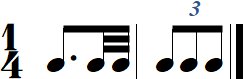
\includegraphics[scale=0.20]{pictures/score5.png}.
 The latter shows a subdivision of the temporal interval $[1, 2[$
 based on the rules from Example~\ref{rules-division}. The first measure ($I_1$)
 results from the successive applications of  rules $\rho_1$ (division in two)
and rules $\rho_3$ (division of the second half) in two. The second measure
is a division in three obtained by rule $\rho_3$. It follows that the notation
defines the sequence of timestamps $0, \frac{3}{4}, \frac{7}{8}, 1, \frac{4}{3}, \frac{5}{3}$.
The distance between $s$ and $t$ is the  pairwise difference between the
timestamps from $s$ and $t$, 0.255.
\endex
\end{example}
